\part{Analysis}
		\chapter{Introduction}
		The aim of this project is to develop a mobile robot capable of utilizing Simultaneous Localization and Mapping, often referred to within robotics as SLAM. SLAM concerns the ability for a robot to move around whilst simultaneously tracking its position and generating a map of the environment it navigates around. This will entail elements of mobile robotics, with regards to the appropriate selection of hardware followed by the assembly of said hardware to create the robot and the development of the software that will run on the mobile platform. Alongside this will be the development of a solution to the SLAM problem to allow the mobile platform to map the environments that it navigates around.
		
		In order to implement this system and solve the presented problems, a clear understanding of the relevant fields needs to be established. The first aim of the analysis is to obtain just that. To do it, there will be a critical review of relevant literature. This will allow a good foundational base to build on, and will allow a greater understanding of how the problems presented by the project are to be solved. From this, solutions as to how these problems will be solved will be ascertained. Following this appropriate tools for the product will be identified, both hardware and software.
		
		\chapter{Mobile Robotics}
		\label{litreview:mobilerobotics}
			\section{Introduction}
			The creation of a ground-based mobile robot will require an understanding of the fundamentals of mobile robotics. The aim of this chapter is to develop such an understanding, looking over the chosen literature and discussing what can be learned for it as well as the steps that would need to be taken for the mobile platform to be fully realised.
			
			\section{Movement}
			\label{litreview:movement}
			This section aims to explore how movement can be achieved in the world of mobile robotics. From this, a greater understanding of robotic movement should be achieved which will aid the robot's development.
			
			At its most basic level, movement in mobile robotics consists of determining a path between the robots current position and its destination. Satisfying any movement tasks in this fashion will involve breaking down movement tasks into motions that accommodate for different constraints, such as the robot's capability and obstacles in the environment. One such constraint that has a significant impact in determining this path is the holonomic (or lack thereof) properties of the robot.
			
			Most conventional vehicles use standard wheels that have only two degrees of freedom. These wheels can either roll forwards or backwards. This means it is a non-holonomic vehicle, which essentially means at any given point in the vehicle's state there are certain directions it cannot travel in. Barraquand and Latombe\citep{barraquand1989nonholonomic}, both experts in their field with Latombe publishing one of the most cited works in the field of mobile robotics, discuss nonholonomic robots and their navigational properties. The example they give to demonstrate non-holonomic constraints is a car. A car is capable of obtaining any position within an environment, but the car wheels are only capable of moving forward or backward. Therefore, the car's achievable velocities at any given point are two dimensional. This is what makes it a non-holonomic vehicle. A common real world example of this being an issue is in parallel parking.
			
			Barraquand and Latombe go on to discuss the problems that non-holonomic navigation possesses. In constructing a collision free path, the first difficulty is in actually determining a feasible path between two points. This is because a straightforward translation of the robot from its initial position to its destination is not always possible. Indeed, Laumond et al\citep{laumond1994motion} in their discussion of the issues with non-holonomic navigation mention that a determined path doesn't always correspond to a trajectory that can be used by the robot. In an article for IEEE, Murray and Sastry\citep{murray1993nonholonomic} demonstrate this by comparing a path generated by a path planner to the actual path that would need to be taken to translate a non-holonomic robot to a destination, seen in fig \ref{fig:generatedpathfailure}.
			
			\begin{figure}[h]
				\centering
				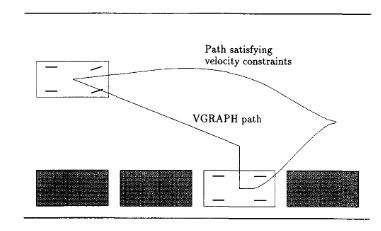
\includegraphics[scale=0.9]{ANALYSIS/generatedpathfailure.png}
				\caption{Generated path ignoring the robot's non-holonomic properties}
				\label{fig:generatedpathfailure}
			\end{figure}
			
			One of the ways in which these problems can be negated is through employing a holonomic vehicle, which would allow it to enjoy the ability to move in any direction regardless of its current position or heading. One of the most popular ways in which vehicles obtaining holonomic properties are constructed is through the use of special omnidirectional wheels.
				
			Watanabe\citep{watanabe1998control}, a Professor at Okayama University's Faculty of Engineering who has published a great deal of work in robotics, discusses a few different variations of these omnidirectional wheels. One of the more popular variations in his discussion is the universal wheel, sometimes also referred to as the swedish wheel or mecanum wheel. This wheel is a larger wheel that has many rollers on the rim which allows the wheel to slide in a direction perpendicular to its motor axis. 
				
			\begin{figure}[h]
				\centering
				\begin{subfigure}{.5\textwidth}
					\centering
					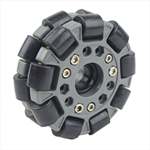
\includegraphics[width=.4\linewidth]{ANALYSIS/90degwheel.png}
				\end{subfigure}
				\begin{subfigure}{.5\textwidth}
					\centering
					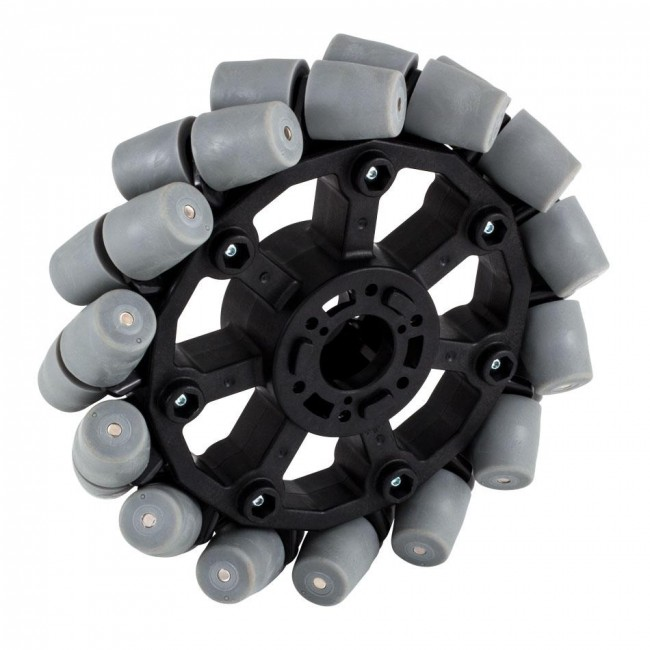
\includegraphics[width=.4\linewidth]{ANALYSIS/45degwheel.jpg}
				\end{subfigure}
				\caption{Wheels with 90 and 45 degree rollers}
				\label{fig:omnidirectionalwheels}
			\end{figure}
		
			The use of such wheels greatly simplifies the robot's movement. Calculated paths between points can be translated much easier into usable commands given the robot's movement freedom, and the number of manoeuvres required is reduced drastically since there is no need for repeated "backing up" movements to adjust the robot's heading.
			
			Watanabe also discusses ball wheels, with one well known implementation of such a wheel being ballbot by Lauwers et al\citep{lauwers2006dynamically}. The ballbot design involves a singular ball instead of any wheels, with legs that can deploy when the robot needs to be stationary. Whilst there are some potential stability issues during movement, with one experiment noting that the robot would lean in the direction of its destination as it traveled, it was still able to resist attempts to tip it over. Whilst interesting, in the context of the project the design of this is a bit too complex for it to be used for a mobile platform.
			
			\section{Rangefinding}
			\label{litreview:rangefinding}
			Used for obstacle navigation and to assist in navigation, mobile robots often feature hardware that allows the robot to observe its surrounding environment. In the context of the project, this will also serve as a way to provide relevant data to allow for mapping. 

			This section aims to explore some of the more common rangefinding techniques by briefly explaining and evaluating them.
			
				\subsection{Infrared}
				\label{litreview:infrared}
				Infrared (IR) sensors work by measuring things via the reflection of infrared light. The sensor will send out some infrared light where it will be reflected off of an obstacle. A reciever will capture this reflected light and depending on factors such as how much light is recieved back and the triangulation of how the light was recieved the presence of an obstacle will be determined. 
				
				In a paper produced for the International Journal of Advanced Robotic Systems regarding the usage of IR in mobile robotics, Do and Kim\citep{do2013infrared} elaborate on some of the advantages of IR. First is their incredibly low cost, with a great number of IR sensors available online for very cheap prices. Websites like RobotShop and HobbyTronics list most of their sensors between \pounds{5} and \pounds{10}. Additionally, IR sensors are able to achieve very narrow beam angle. This allows for precise detection, and can mean IR sensors excel where other sensors such as Sonar encounter environmental limitations such as spaces where wave reflection might cause inaccurate readings. 
				
				These benefits have been enough to see IR's usage robotics projects. Malik and Yu\citep{malik1992infrared} for example utilised a ring of IR detectors for performing obstacle detection with an autonomous robot. Their implementation of it was quite successful, the robot demonstrated basic navigational abilities such as moving through doors and finding its way around unknown environments, successfully avoiding obstacles in the process. Dang and Suh\citep{dang2011human} implemented a tracker using IR. In their experiments, their created devices succeeded in tracking humans and demonstrated an error (tracking inaccuracy) of less than 1.5cm when it was used for real world applications such as following supermarket carts.
				
				IR has some downsides however. First, infrared sensors have both a maximum and a minimum range. Not only does the maximum range need to be factored in as sensor will struggle to pinpoint the location of light that has been reflected at a large range, but the sensor will also struggle to 'see' very close obstacles. Lee and Chongp\cite{lee2011low} in their discussion of the different rangefinding techniques touch on IR's faults and mention that IR can have trouble with object detection depending on the colour of the object reflecting the IR light.
				
				\subsection{Ultrasonic}
				\label{litreview:ultrasonic}
				Ultrasonic sensors function by sending out ultrasonic pulses and measuring the amount of time it takes for these pulses to bounce back. 
				
				Like IR, Sonar sensors tout a relatively low price range towards the low end, with sites like HobbyTronics and RoboShop featuring sensors as cheap as \pounds{6}.  This would allow for a cheap way to implement coverage around the entirety of a robot, as multiple sensors could be attached and configured on the outside of the robot's chassis. Sonar's sound based nature means it isn't negatively affected by aspect such as heat or colour. 
				
				Sonar isn't without problems however. In an article for IEEE, Borenstein and Koren\citep{borenstein1988obstacle} discuss some of the drawbacks of ultrasonic range finders during their foray into using it for obstacle detection. The first issue was that detection could be very unreliable depending on the angle the sonar energy hit the surface at. Parallel surfaces were detected without issue but more perpendicular surfaces caused a lot more of the sonar energy to be scattered and resulted in the detection being less reliable. This issue appears to get worse the smoother a surface is, with things like polished wood and plastics giving the worst results. Another problem was accuracy. Depending on the sensor's orientation and the angle at which an obstacle reflected the sonar energy, the received readings could be incredibly noisy. As well, sensors sending and receives pulses in close proximity to each other can have issues with interference. Whilst the article is 30 years old, the papers mentioned previously in the discussion of IR - despite being significantly more recent - still noted similar drawbacks to the use of sonar in their discussion of it\citep{do2013infrared}\cite{lee2011low}. We can infer from this that these issues are most likely due to the way in which sonar works, rather than the technological ability of the sensors used in the experiments.
				
				\subsection{LIDAR}
				\label{litreview:lidar}
				LIDAR (Light Detection And Ranging) is a technology that uses light sensors to measure distances between the sensor and the target object. It achieves this by sending out light pulses which bounce off of objects back at the sensor where they are collected.
				
				LIDAR's biggest strength is arguably the accuracy that can be achieved compared to other rangefinding techniques, which has led to its adoption for projects where accurate measurements are needed. One field that LIDAR enjoys much usage in because of this strength is forestry. Dubayah and Drake\citep{dubayah2000lidar} mention the strengths of LIDAR for measuring forest features such as canopy heights, with similar praises for the accuracy are given by Lim et al\citep{lim2003lidar} investigation into LIDAR's effectiveness for measuring forest structure. Some commercially available sensors boast very impressive statistics, with some ranges exceeding 10 metres whilst providing several thousand samples per second with 360 degree coverage \citep{slamtecA1M8}. Some of these sensors also feature SDKs (Source Development Kits), meaning the core sensor functionality will be accessible straight away allowing development to focus on the robot's logic rather than being bogged down in the belt and braces implementation of preliminary functionality. 
				
				All of these features come with an expected financial downside however. These features are expensive, with some sensors being as high as \pounds{350}. Even lower end options with much smaller sensors that don't offer full 360 degree cover can cost up to \pounds{40}.
				
		
		\chapter{An Investigation Into SLAM}
			\section{Introduction}
			The development of a moving robot is only one half of the end product. As previously mentioned in the project's Terms of Reference the purpose of this project is also to develop a robot that is capable of self navigation and mapping. In order for this to be possible, the robot must be capable of using observations about its environment to build a map. Not only that, but it also must track its own location within this environment. This chapter aims to explore SLAM, a computing problem with research and implemented solutions that deal with exactly that.
		
			\section{What is SLAM?}
			SLAM stands for Simultaneous Localization and Mapping, and is something sometimes employed by mobile robots. Localization refers to the ability for the robot to be aware of its location within an environment, for example knowing where it is within a room. Mapping simply refers to building a map of the environment, such as the room the robot is in. SLAM is performing both of these tasks at the same time. Durrant-Whyte and Bailey\citep{durrant2006simultaneous}, both academics that have done extensive work in the field of mobile robotics, best sum it up as the ability for a mobile robot to be placed at an unknown location in an unknown environment and then both create a consistent map of the environment and be able to accurately determine its location within this map. Similar definitions can also be found in other articles \citep{choset2001topological, dissanayake2001solution}.
		
			\section{Uses of SLAM in Industry}
			There are a myriad of potential uses for SLAM, many of which can be seen within the wider industry. Commercially it has been used for products such as vacuum cleaners, Dyson for instance has a small automated vacuum cleaner called the 360 Eye which employs SLAM techniques to map the areas that it moves around and cleans. SLAM has seen many uses in archaeological contexts owing to its ability to perform exploration without risk to human life, one team \citep{clark2008archaeology} developed an underwater robot that used SLAM in order to map underwater cisterns that had been built thousands of years ago. The uses have not gone unnoticed by larger organisations. One of the research organisations within the USA's Department of Defense has held challenges (known as the DARPA Grand Challenge) offering cash prizes as incentives to create high value research. These challenges involve organisations submitting cars that are timed as they race around certain environments. NASA have also made use of it in the past, in 2007 they used an autonomous underwater robot \citep{carnegie2007sinkhole} employing SLAM to go to the bottom of the world's deepest sinkhole. The robot used sensors to generate a sonar map of the sinkhole's inner dimensions 318 meters below the surface.  The drone also tested technologies that could be used in other more extreme underwater environments such as the oceans under the crust of Europa, one of Jupiter's moons. This has led to increased interest being expressed in using SLAM for planetary rovers, which would allow for the mapping and navigation of different planet surfaces.
			\medskip
		
			\section{The SLAM Problem}
			\label{litreview:slamproblem}
			Let's use some key notations to help break down the essentials of the SLAM problem. \newline
			\textbf{t} - Current time. \newline
			\textbf{x\textsubscript{t}} - Location and orientation of vehicle. \newline
			\textbf{u\textsubscript{t}} - Control vector, for example drive forward 1 metre.  \newline
			\textbf{m\textsubscript{t}} - True location of \textit{i}th landmark within the environment. \newline
			\textbf{z\textsubscript{t}} - Observation of \textit{i}th landmark taken at time \textit{t}.\newline
			
			From these notations we can derive some sets. \newline
			\textbf{x\textsubscript{0:t}} = $\lbrace$ \textbf{x\textsubscript{0:t-1}}, \textbf{x\textsubscript{t}} $\rbrace$ - History of all vehicle locations. \newline
			\textbf{u\textsubscript{0:t}} = $\lbrace$ \textbf{u\textsubscript{0:t-1}}, \textbf{u\textsubscript{t}} $\rbrace$ - History of odometrical information pertaining to teh robot's movement. \newline
			\textbf{m} = $\lbrace$ \textbf{m\textsubscript{1}}, \textbf{m\textsubscript{2}}, ..., \textbf{m\textsubscript{n}}$\rbrace$ - Set of all landmarks. \newline
			\textbf{z\textsubscript{0:t}} = $\lbrace$ \textbf{z\textsubscript{0:t-1}}, \textbf{z\textsubscript{t}} $\rbrace$ - Set of all landmark observations. \newline
			
			Ultimately we want to use the robot's control inputs and observations to receive a map of the environment and the robot's path.
			
			\begin{figure}[h]
				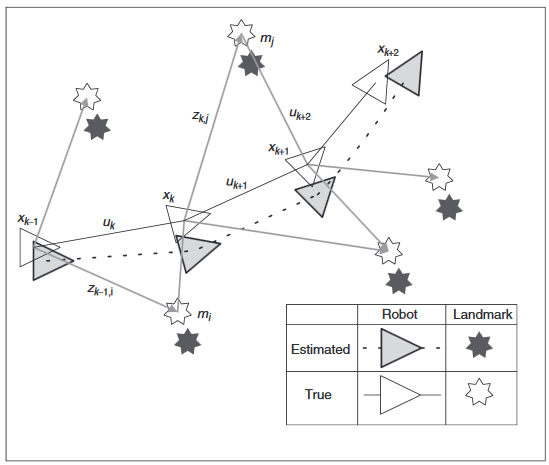
\includegraphics[scale=0.65]{ANALYSIS/slamdiagram.png}
				\caption{The SLAM problem illustrated \citep{durrant2006simultaneous}}
				\label{fig:slamillustration}
			\end{figure}
			
			SLAM is generally approached probabilistically. This means that the attempted solutions factor in uncertainties within the data. Therefore, solutions to the SLAM problem will not act with exact certainties. For example, rather than saying the robot is in an exact location we would treat it as a general location it is the most likely to be in. We want the probability distribution to be an estimation of current vehicle location and landmarks based on landmark observations and control inputs or odometrical data. 
			
			There are variations within the SLAM problem however. At a broader level, SLAM problems generally come in one of two flavours. These are full SLAM and online SLAM. 

				\subsection{Full SLAM}
				\label{litreview:slam:fullslam}
				Full SLAM involves using landmark observations and data relevant to discerning the robot's current position in order to determine the robot's entire path. It can be written as such -
				
				p(\textbf{X\textsubscript{0:t}}, \textbf{m} $\mid$ \textbf{Z\textsubscript{0:t}}, \textbf{U\textsubscript{0:t}})
				
				We want the probability distribution (essentially the estimation of the robot's current position) to be an estimation of what is on the left (current vehicle location and landmarks) based on what's on the right (landmark observations and control inputs).
				
				\subsection{Online SLAM}
				\label{litreview:slam:onlineslam}
				Online SLAM differs slightly in that it seeks to determine the robot's current location rather than the robot's entire path. It can be written as such - 
				
				p(\textbf{x\textsubscript{t}}, \textbf{m} $\mid$ \textbf{Z\textsubscript{0:t}}, \textbf{U\textsubscript{0:t}})
				
				Compared to the previous notation used in \ref{litreview:slam:fullslam}, this probabilistic estimation only estimates the robot's position (x) at the current time (\textsubscript{t}) rather than the robot's full historical path.
				
				\subsection{SLAM Taxonomy}
				The possible differences in the SLAM problem don't end there. Depending on different factors there are also different sub approaches to the SLAM problem. Below are some common variants.
				
					\subsubsection{Volumetric versus Feature-Based}
					Volumetric SLAM samples the map as a resolution high enough to allow a photo realistic reconstruction of the environment \citep{thrun2008simultaneous}. The map gained from this is generally high dimensional, but as the area increases in size and scale the map becomes significantly more complex. Feature-based SLAM simply extracts key features from measurements, with the map being solely made up of these features. This might be used if it is decided that only key features are of interest or if large parts of the mapped space are empty, as volumetric SLAM in these cases would be storing voxels that hold no geometric data of significant value \citep{vespa2018efficient}. As you would expect, this is quicker and more efficient but discards a lot more data than volumetric. 
					
					\subsubsection{Topological versus Metric}
					Topological SLAM captures key places and their connectivity to other measured locations. Metric SLAM attempts to model the environment using geometrically accurate positioning. Metric SLAM would show the accurate positioning of various environmental features, topological would show them in relation to each other (e.g. place A is adjacent to place B) \citep{thrun2008simultaneous}. A good analogy would be a bus route map (topological) that displays the different stops versus showing the bus' actual route on a geographical map of the area (metric).
					
					\subsubsection{Known versus Unknown Correspondence}
					This entails relating the identity of sensed landmarks to other sensed landmarks. In known correspondence the identity of the landmarks is known, if a landmark is observed and then the robot moves and observed another landmark, the identity of the landmarks being known would let us to determine if this landmark observation is the one we saw before or a newly observed one. Unknown correspondence would simply mean that in this situation we wouldn't know.	
					
					\subsubsection{Static versus Dynamic}
					Static and Dynamic here refers to the environment. Static SLAM algorithms assume that no changes will take place in the environment whereas Dynamic SLAM methods allow for these changes to take place.
					
					\subsubsection{Small versus Large Uncertainty}
					The ability to represent uncertainty is another aspect. Some SLAM approaches will assume a very low uncertainty in the robot's location estimation. This might be when the robot is moving up and down a simple path, as it's much easier to guess where it's likely to be. Large amounts of uncertainty might occur however in more complex environments where locations can be reached from multiple different directions, or if the robot starts travelling in more complex paths that intersect with each other.
					
					
					\subsubsection{Activate versus Passive}
					Active SLAM involves the robot actively exploring its environment whilst it builds a map of it. Passive SLAM is when the SLAM algorithm is purely used for observation, with some other entity controls the robot's movement. 
					
					\subsubsection{Single-Robot versus Multirobot}
					Single-robot simply refers to SLAM happening only on a single platform. Multirobot SLAM (sometimes known as cooperative SLAM) involves multiple robots often communicating with each other to merge their maps into a larger collective model. 
				
					\medskip
					There are multiple different paradigms that can be used to solve the SLAM problem, and each of these paradigms has many different implementations. One technique that has seen usage for solving the SLAM problem in autonomous mobile robotics is the Canonical Scan Matcher, generally referred to as CSM. This is the solution that we will be looking to implement for the project.

			\section{A Look At A Potential Solution}
				\subsection{Introduction}
				As previously discussed there are a myriad of variations on the SLAM problem, and there are a few different paradigms used to implement solutions to it. During some preliminary research, one method of SLAMming came up that seemed like it would be suitable for the project called CSM.
				
				\subsection{CSM}
				CSM is an open-source C implementation of an ICP variant known as PlICP. It has seen usage for industrial prototypes of autonomous robotics, one of the most notable examples of this being Kuka, a German manufacturer of industrial robotics. It isn't quite a fully fledged SLAM solution, instead performing pairwise scan-matching on scan data that is fed into it. Before the PlICP algorithm it is based on can be explained, we must first look at the base ICP algorithm.
			
					\subsubsection{ICP}
					ICP stands for Iterative Closest Point, and it refers to an algorithm that attempts to minimize the difference between two clouds of points, something known as point matching or point set registration. In essence, it means getting one set of points aligned to another set of points. Besl and McKay present the algorithm as a statement \cite{besl1992method} in their paper, and ICP is shown in terms of C++ in the Mobile Robot Planning Toolkit \citep{mrpt2013icp}. 
					
					We first of all have a source map, and then we have a map that we wish to align to it which we will refer to as the reference map. We then go through each point in the source map and which point in the reference map is the closest to it. We then determine a transformation which would minimize the mean squared error (the average squared difference) between the two points before applying this transformation to the reference set and then going through this set of steps again. This is repeated until a the mean squared error falls below a certain threshold.
					
					\subsubsection{PlICP}
					Censi explains PlICP in a series of steps \citep{censi2008icp}. To start with, we take a reference scan, a second scan and a first guess for the translation needed to try and match the two maps. We then generate a polyline of the reference map by connecting sufficiently close enough dots (using a threshhold). Following this, a loop similar to the one in the base ICP algorithm begins.
					
					We first determine the coordinates of the second scan in the first scan's frame of reference using our initial translation guess. Then, for each point in the second scan, we determine the two closest points to it in the first scan. We trim any outliers within these matches, and use the sum of the squares of the distances from the points to the line containing the matches two points to find the error function. PlICP then uses an algorithm in order to minimize this error function which we now use as our translation guess. This new guess is used on the next iteration of the algorithm. This loop continues until either we have a convergence between the maps or a loop is detected as no further progress is being made.	
					
			\subsection{Suitability of CSM}
			Firstly we can see that CSM is a pure C implementation of the previously described algorithm. This is excellent for the project, not just for the benefits of C such as it being a relatively quick language but also because it should be directly usable with an embedded board which would be the ideal choice for controlling the robot. Had it been in any other language we might have needed to use some sort of shared library to get it to work which likely would have slowed things down and potentially made the robot less effective. 
			
			CSM is however not a product of a professional company dealing in these matters, its open source nature could put some doubts with regards to its usefulness or reliability. However, it was developed by Dr Andrea Censi, someone who is a Deputy Director for the Chair of Dynamic Systems and Control at ETH Zurich meaning it is far from an amateur project. As previously mentioned as well it has been adopted by the German robotics company Kuka, so clearly it has enough merit to be used at the industrial level. Ultimately it would appear CSM is an ideal choice for the robot's localization and mapping functionality.
					
			\section{An Investigation Into SLAM - Conclusions}	
			First and foremost we can safely establish that the SLAM problem is what we are addressing with regards to the implementation of the robot's ability to track its own location whilst mapping its environment. In addition to this we understand the fundamentals of the SLAM problem. This will massively benefit development, as being aware of having to store details internally such as wheel revelations gained via odometric sensors will allow us to cut down on time spent during development having to rewrite core pieces of functionality to make room for this. 

		\chapter{Product Requirements}
		\label{requirements}
		Based on the different aspects of mobile robotics and SLAM that have been looked at as well as preliminary project objectives outlined in the Terms of Reference, we can outline the basic product requirements that will need to be achieved in the course of the product's development.
		
			\section{Functional}
			\label{requirements:functional}
			\begin{itemize}
				\item The robot must be capable of movement
				\item The robot must be capable of observation
				\item The observational data must be processed into a map
			\end{itemize}
			
			\section{Non-Functional}
			\label{requirements:nonfunctional}
			\begin{itemize}
				\item \textbf{Build Quality} - The robot should be built to an acceptable standard. Wires should be managed to ensure the robot's function isn't impeded by them (e.g. getting stuck in the wheels) and components should stay inside the chassis during the robot's operation.
				\item \textbf{Functional Speed} - The observation and map generation should be done within an acceptable time. The robot shouldn't take more than 10 seconds to save readings, and it shouldn't take more than 30 seconds to generate a map from the readings once they have been acquired.
				\item \textbf{Adaptable Mapping} - To ensure the robot maps correctly, the mapping should be tested against a few different layouts. This will ensure the implemented method of mapping can successfully adapt to and map new environments.
				\item \textbf{Reliable Mapping} - When mapping the same environment multiple times, the robot's produced maps shouldn't differ too much. Repeated testing in the same environment will be carried out to ensure produced maps are consistent.
			\end{itemize}
		
			\section{Security}
			There are no security requirements for the system.
		
		\chapter{Review of Tools and Techniques}
		This chapter aims to focus on evaluating the potential tools and techniques that will be employed for the project's implementation. It will explore appropriate potential hardware and software, arriving at a conclusion along with an explanation as to why a certain tool or technique has been chosen.
			\section{Tools}
				\subsection{Chassis}
					A few of the different chassis found during the preliminary research will now be evaluated to find which would be the most suitable for the project.
					
					\subsubsection{4WD 58mm Omni Wheel Arduino Robot - \pounds{260.78}}
					\begin{figure}[h]
						\centering
						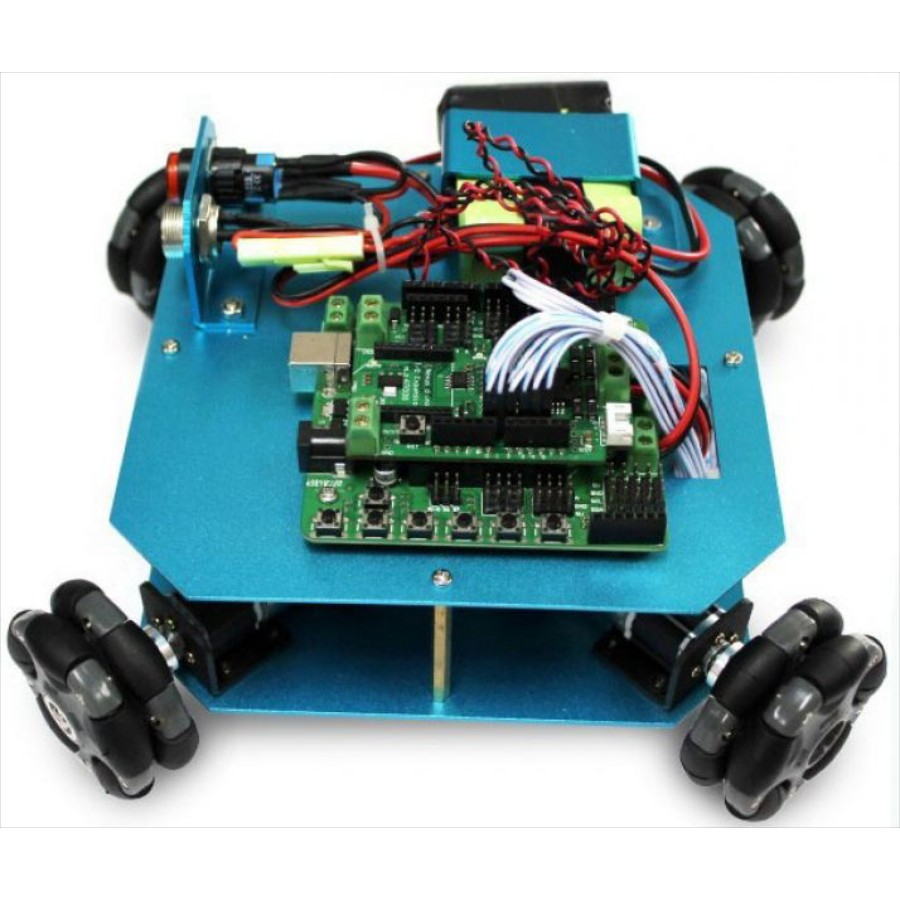
\includegraphics[width=.3\linewidth]{ANALYSIS/4wdomnidirectionalarduino.jpg}
						\caption{4WD Omni-Directional Robot Chassis}
						\label{4WD Omni-Directional Robot Chassis}
					\end{figure}
					This chassis features four of the aforementioned omnidirectional wheels along with appropriate motors. The motors have encoders with them which record wheel revolutions, allowing us to use odemetric measurements should we connect these encoders to the microcontroller. This kit includes the microcontroller which is an Arduino 328, as well as a nickel metal hydride battery and an appropriate charger. The kit also includes an IO expansion board which would allow us to connect more external devices\cite{4wdArduinoChassis}.
					
					Whilst it would be useful to have most of the equipment decisions done for us, some of this is not necessary. The IO expansion board for example will most likely be needed, as all we're really interested in adding is a sensor for observations. As well, the price of the kit is quite high given we would also need to purchase a LIDAR sensor on top of it.
					
					\subsubsection{3WD 48mm Omni-Directional Triangle Mobile Robot Chassis - \pounds{114.34}}
					\begin{figure}[h]
						\centering
						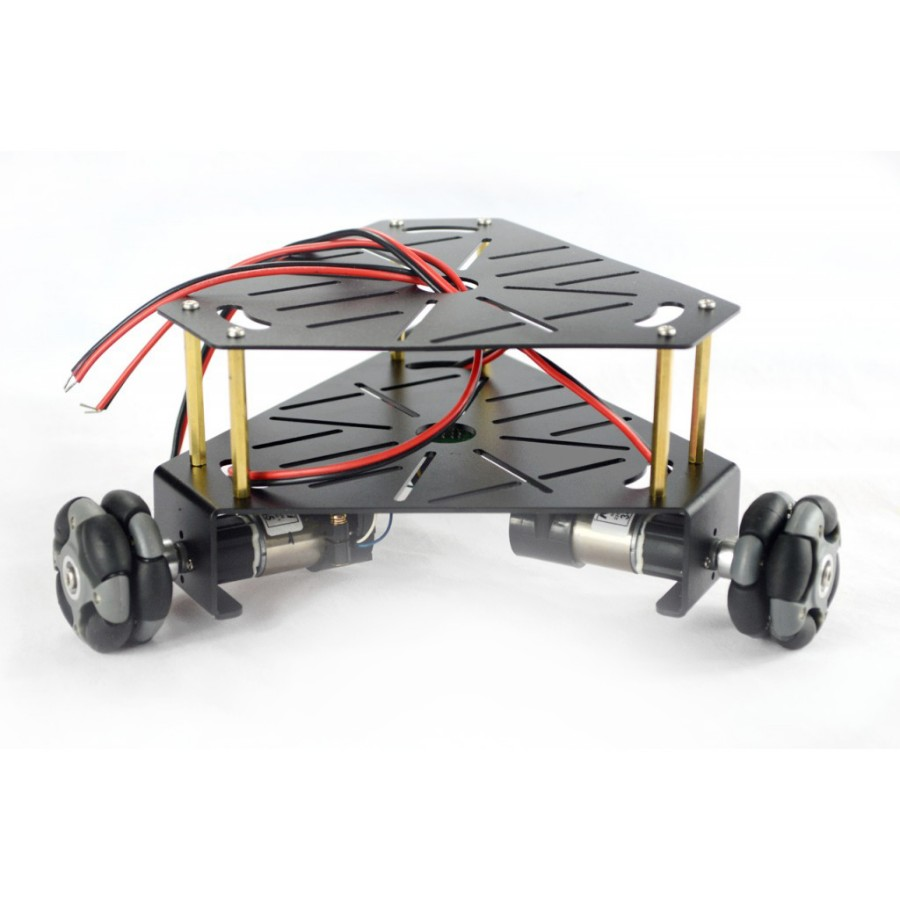
\includegraphics[width=.3\linewidth]{ANALYSIS/3wdomnidirectionalchassis.jpg}
						\caption{3WD Omni-Directional Robot Chassis}
						\label{fig:2}
					\end{figure}
					Unlike the previous chassis this one features only three wheels rather than four. This is still enough to achieve freedom of movement however. Whilst it doesn't include the additional pieces of the kit the other does (such as a microcontroller) we still have our wheels, a supporting structure and appropriate motors with encoders that will provide us with odometric data. There is plenty of room in the middle for items such as our microcontroller and a power source, and the top plate is an ideal mounting point for our sensor\cite{3wdomnichassis}.
					
					Whilst still a bit expensive, the chassis is still on the cheaper side compared to the previous one and some cost is expected to be incurred given that a 12v DC motor with an encoder can cost around \pounds{30}. One issue encountered while looking for an appropriate robot chassis is that the majority on sale seem to already include microcontrollers and sensors, which launches their price up and also removes a lot of the choice from the product. Looking around the RobotShop and HobbyTronics website for just an empty chassis only yielded this product. Based on these factors, this chassis will be the one used for the product.
			
				\subsection{Microcontroller}
				The main functioning of the robot will need to be controlled by a suitable microcontroller. Something relatively small and cheap with sufficient GPIO pins should work fine.
				
					\subsubsection{Arduino Uno Rev3 - \pounds{20.80}}
					\begin{figure}[h]
						\centering
						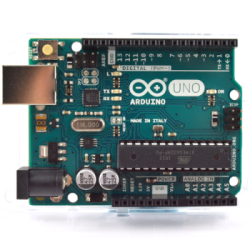
\includegraphics[width=.3\linewidth]{ANALYSIS/arduinounorev3.png}
						\caption{Arduino Uno Rev3}
						\label{fig:arduinounorev3}
					\end{figure}
					First and foremost the Arduino features a very small form factor, which is good for the robot as less space being taken up by the microcontroller means there is more room for proper cable management and other components. As well, it has several I/O pins which should accommodate any sensor that is used for observation. It also sits at a relatively low price point, costing around \pounds{20} on sites such as rs-online\cite{arduinounorev3}. Unfortunately the technical specification is somewhat underwhelming, as it only boasts 30 kB of available memory with an also slow clock speed of 16MHz\cite{arduinounorev3docs}. The low memory and clock speed could present issues in operation, as it could result in insufficient space to store readings as well as a potentially long time to carry out any read/write tasks.
				
					\subsubsection{FRDM-K22F - \pounds{23.57}}
					\begin{figure}[h]
						\centering
						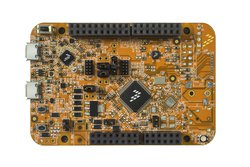
\includegraphics[width=.3\linewidth]{ANALYSIS/k22f.png}
						\caption{FRDM-K22F}
						\label{fig:k22f}
					\end{figure}
					The K22F features higher specs than the Arduino, with 128kB of RAM and a 20MHz CPU. It also features a small form factor as well as an impressive 40 GPIO pins, which will easily accommodate any peripherals that the robot will make use of. The fact that the microcontroller is an arm Mbed product also allows it to make use of the online Mbed compiler as well as the Mbed SDK which could aid in development\cite{frdmk22fdocs}. Unfortunately the board is not featured on any common vendor websites based in the UK, with most sellers being based in the US which means it could take a while to arrive. Vendors that ship it from the US cost around \pounds{23} to \pounds{25}\cite. In addition, it somewhat pales in comparison to a more sophisticated model which can be acquired at no cost from the University's loan office.
					
					\subsubsection{FRDM-K64F}
					\begin{figure}[h]
						\centering
						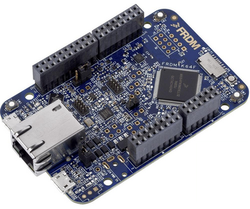
\includegraphics[width=.3\linewidth]{ANALYSIS/k64f.png}
						\caption{FRDM-K64F}
						\label{fig:k64f}
					\end{figure}
					Essentially an upgraded version of the FRDM-K22F, the K64F features more RAM and a faster CPU than its more budget oriented counterpart. There are also a few additional peripherals that come already attached, such as a Micro SD-Card reader allowing our robot to read and write to an external storage medium\cite{frdmk64fspecs}. It too boasts all of the accessibility to the online compiler and Mbed SDK that the K22F does. These features combined with its free availability at the University's loan office make it the ideal choice for the project.
			
				\subsection{Rangefinder}
				Based on the discussion regarding the various rangefinding techniques in the mobile robotic's section, it was decided that LIDAR, whilst the most expensive, seems to be the most appropriate for the project. This was primarily due to its ability to be unaffected by poor light levels or other sensors, as well as available sensors that feature pre-implemented functionality. In addition, the high accuracy of LIDAR mentioned by a few papers in \ref{litreview:lidar} will allow the created map to possess a high level of detail. Here we will look at a few different LIDAR sensors that could be suitable for the project.
				
					\subsubsection{RPLIDAR A2M8 360 Degree Laser Scanner - \pounds{301.43}}
					\begin{figure}[h]
						\centering
						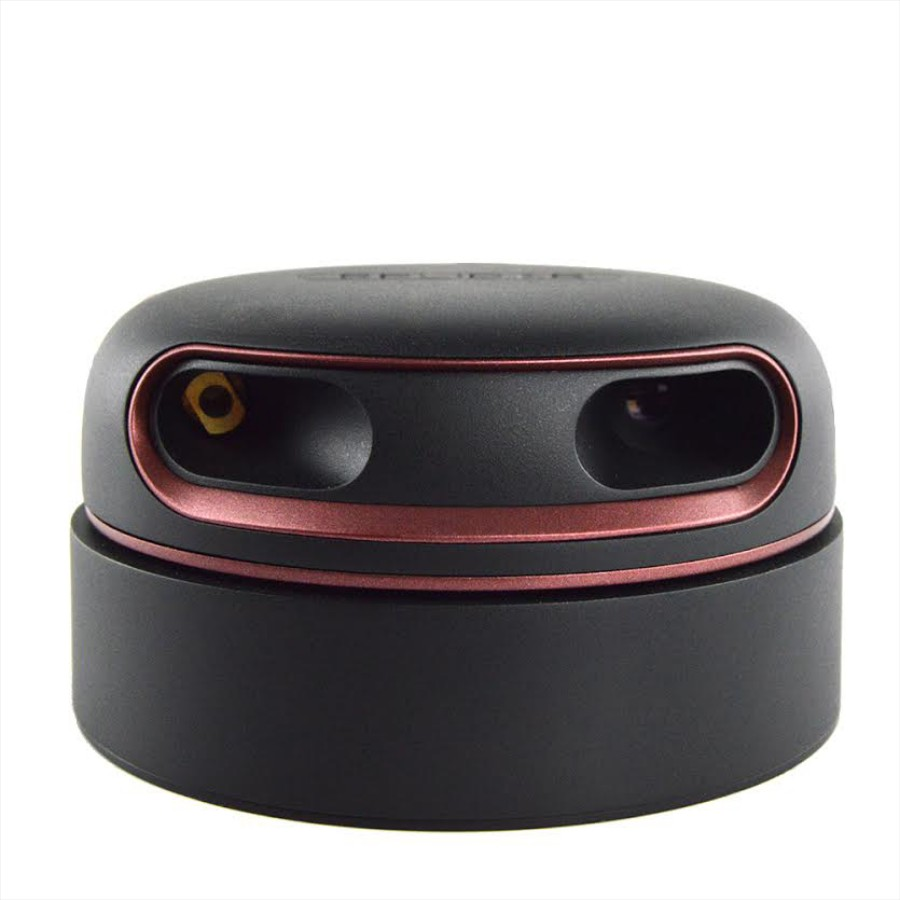
\includegraphics[width=.3\linewidth]{ANALYSIS/rplidara2.jpg}
						\caption{RPLIDAR A2M8}
						\label{fig:rplidara2m8}
					\end{figure}
					The RPLIDAR A2M8 uses the previous described LIDAR triangulation system, and outputs scan data at 8000 samples per second\citep{rplida2m8docs}. It outputs this data via a relevant communication interface, representing scans as distance (what distance between the sensor and the measuring point) and heading (the heading angle of the measurement). It also includes a start flag in its measurement signalling the start of a new scan, which would likely come in useful for processing the scan data as we could simply check this flag to see if incoming data is from a new scan. One of the biggest advantages to employing this sensor would be the SDK it comes with. With full documentation\cite{rplidarsdkdocs}, the SDK allows us to access the sensor's entire functionality straight away. It has appropriate methods for beginning the scanning session, ending it and checking sensor health as well as a few other things. This would save a lot of time in the project as we could focus on logical implementation rather than creating the prerequisites that will be needed for the sensor to do what we need it to do.
					
					The major downside to all of these advantages however is the cost. Sitting at just above \pounds{300}, this is an incredibly steep price for the project if we factor in the cost of the other equipment such as the chassis. This problem leads us to the final choice.
					
					\subsubsection{RPLIDAR A1M8 360 Degree Laser Scanner - \pounds{93.54}}
					\begin{figure}[h]
						\centering
						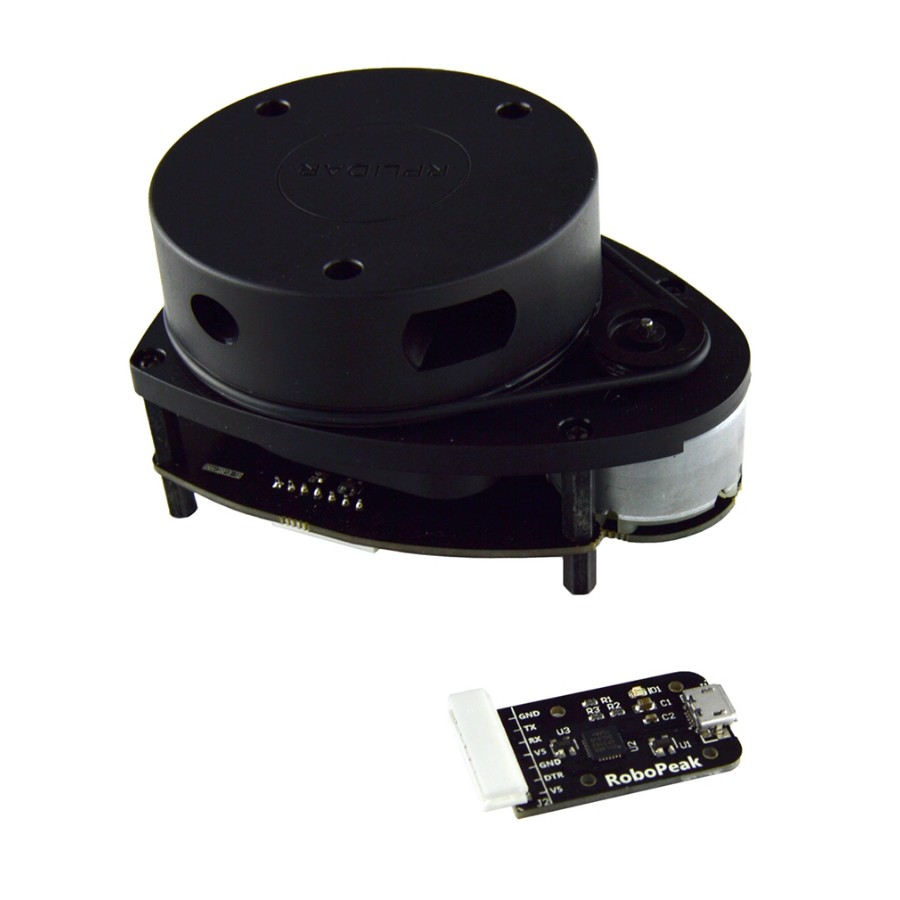
\includegraphics[width=.3\linewidth]{ANALYSIS/rplidara1.jpg}
						\caption{RPLIDAR A1M8}
						\label{fig:rplidara1m8}
					\end{figure}
					Essentially a less sophisticated version of the previous sensor, this iteration of the M1 LIDAR sensor still offers us a 4000 - 8000Hz sample frequency as well as the previously mentioned SDK\cite{rplidara1m8datasheet}. Among a few other things, the key differences here are that we have a slightly slower scan frequency (1 - 10Hz vs the A2's 5 - 15Hz) and a few pieces of SDK functionality that aren't available on the less advanced firmware. The key change is that we lack the express scan function, which is similar to the regular scan but it performs at the highest sampling rate the sensor can use. The upside however is a lower price point\cite{rplidara1m8price}.
					
					These downsides are negligible with our product however, ultimately as long as we can easily get observational data at a reasonable rate the project benefits hugely. This functionality at the far more agreeable price point makes this the sensor of choice for the robot.
				
				\subsection{Software Framework}
				With regards to the software that will be running on the robot itself, it makes sense to implement it as an operating system. Appropriate tasks will be made to deal with things such as the robot's movement and interaction with the LIDAR sensor. This section aims to explain our potential options for how this operating system will be implemented before coming to a conclusion on which of the options will be used and why.
				
					\subsubsection{MBED RTOS}
					The MBED Real-Time Operating System is an open source operating system for platforms using Arm microcontrollers. It is specifically designed for IoT (Internet of Things) devices, which the OS documentation\citep{mbedrtosdocs} define as low-powered, constrained devices which require access to the internet.
					
					Aside from the usual features you'd expect from an operating system (threads, semaphores, etc), MBED OS also features C++ based network sockets for the sending and recieving of data, network interface APIs for interfacing with things such as ethernet or wi-fi as well as bluetooth support. One aspect of the Terms of Reference dealt with precisely how map data would be handled, with two of the three options involving wireless transmissions. Should the project go in this direction, MBED OS' numerous APIs for dealing with this would be immensely helpful. All of this may be overkill however, communication without the use of these APIs isn't impossible and if we don't use wireless communication then all of these features will be of no use anyway. Should another method of dealing with map data such as locally storing it, a much simpler OS would be more appropriate.
					
					\subsubsection{\textmu C/OS-II}
					\textmu C/OS-II (which will hereon be referred to as Micro C OS) is a very simple real time operating system designed for use with embedded systems. Labrosse\citep{labrosse2002microc} discusses a number of different features of Micro C OS in the documentation in addition to ones you would typically find in an operating system (semaphores, task management, etc). Labrosse discusses how Micro C OS is able to be used on a wide variety of microprocessors owing to its design, allowing it to be highly portable. In addition, Micro C OS's scalability is discussed, allowing for only the services required in the operating system's host application to be used. This feature in particular would come in useful for the project given the use of a microcontroller, as it would allow us to cut down memory usage to only what we need which should help performance issues from arising.
			
			
			\section{Techniques}
				\subsection{Acquiring Scan Data}
				One aspect that needed to be addressed was how the observational data was actually dealt with. Once the LIDAR is taking observations, how does this data find its way back to a terminal where it can actually be used? In the Terms of Reference, a few different options were considered. These were either storing the data locally on the drone or wirelessly transmitting the map data. What follows is a brief investigation into which of these two approaches would be the most viable.
					
					\subsubsection{Local Storage}
					One approach is for the observational data taken by the sensor to be stored on a local storage medium. The K64F features a Micro-SD card socket, and given that the Micro-SD card can be obtained from the University's loans office this approach would incur no extra cost or time spent waiting for a delivery. Mbed features an SDFileSystem library\citep{sdfilesystemlibrary} which would allow for a quick implementation of this on the software side of things. The use of local storage would also allow for the robot's range to be essentially unlimited as well. 
					
					The speed of this approach should be considered. Given how it's likely the robot will take at least a few thousand readings based on the chosen sensor's sample rate, writing thousands of values to the SD Card might end up taking a while. Given the instant accessibility of this equipment, a few tests were carried out to see if these issues might present a problem. 
					
					A simple program was used that measures how much time it takes for a section of code to execute. A 60MHz timer was started and stopped before and after the execution of code that involved writing 16000 samples to a file on the Micro SD-Card, which given the LIDAR's sampling rate of 4000 - 8000 was a few second's worth of scan data. An actual time in microseconds for the software's execution can be determined by dividing the elapsed clock cycles by the timer's clockrate in MHz. This code was ran multiple times and the mean clock cycles for each execution time was stored. Table \ref{table:filewritetests} shows the results of these tests.

					\begin{table}[h!]
						\centering
						\begin{tabular}{|| l | l ||} 
							\hline
							Test & Time in Seconds to Write Data \\ [0.5ex] 
							\hline
							1 & 7.9 \\ 
							2 & 7.9 \\
							3 & 7.7 \\
							4 & 7.7 \\ [1ex] 
							\hline
						\end{tabular}
						\caption{Time taken to write 16000 dummy samples to the Micro SD-Card}
						\label{table:filewritetests}		
					\end{table}
					Writing several thousand samples to the SD-Card won't be an issue, and the created files seemed to be around 250kB meaning the 8GB SD-Cards that can be freely obtained from the University's loans office will have more than ample storage capacity.
					
					\subsubsection{Wireless Transmission}
					In order to transmit the map data, some form of transmitter will likely need to be added to the microcontroller. An RF (Radio Frequency) transceiver could be added to the microcontroller allowing it to transmit and receive radio signals. The K64F features headers for use with 2.4GHz radio add on modules, and a nRF24L01P Nordic transceiver can be obtained very cheaply for just a few pounds online. The Mbed website also has a library\citep{nRF24L01Plibrary} for this transceiver which would allow for interaction with it to be relatively straight forward. Data transmission shouldn't be a problem either. The transceiver's data sheet\ref{nRF24L01Pdatasheet} says that the transceiver has a minimum transfer rate of 250kbps. The A1M8's documentation\cite{rplidara1m8datasheet} mentions distance and heading as two attributes of the working mode's data output. It also mentions the sensor's 4000 - 8000hz sampling rate. If we assume the sensor is always going to be working at the highest sampling rate and that both the angle and distance values are stored as floats, then every second we recieve 16000 float values (8000, the sampling rate, multiplied by two since each scan will feature two floats to be stored). Since each float is four bytes that means to acquire this second's worth of scan data, the transceiver would need to transmit 64000 bytes, or 64 kilobytes. Given the worst case scenario transmit speed of 250kb/s this would be done in less than a second, so we shouldn't have any trouble transmitting as much observational data as we might need.
					
					The problem here though is that having just a transceiver on the robot's microcontroller wouldn't be enough for interaction with it, a second microcontroller would need to also have a radio chip soldered on so that something could actually receive transmissions. Attempting to get pairs of microcontroller listening to each other presents problems in of itself, and as well the use of a radio would mean the robot's range is potentially limited.
					
					\subsubsection{Deciding on an Approach}
					Whilst the wireless transmission approach boasts more initial range and and allows for the robot's observational data to be acquired much quicker, the readily available components, reduced setup time and greater internal storage offered by the Micro SD-Cards space make it the technique of choice for dealing with the observational data. Despite this, the ability for a transmitter to send a simple confirmation signal indicating the robot isn't stuck or experiencing problems would greatly augment the robot's ranged capabilities. Should time allow it, this could be a good addition to the robot once the rest of the system is in place.
				
				\subsection{Dead Reckoning}
				Odometry is the usage of data from motion sensors to estimate an object's position. One such implementation of this that will be looked at for the project is dead reckoning. Dead reckoning tracks the robot's position by using data from wheel encoders that count the number of wheel rotations performed during operation. From this, the internal tracked position of a robot can estimate its new position after periods of movement. Given that the chassis being used for the project has wheel encoders as part of the wheel motors, this approach would allow us to perform odometry without needing the use of additional kit. Dead reckoning is not without issues however. Most pressingly it does not account for wheel slippage. If the robot has a poor grip on the ground and the wheels slip, then the wheel rotation doesn't accurately correspond to the robot's location \citep{choset2001topological}. These issues would compound as well. As more and more slippage happens, the robot's internal position would become less and less accurate to where it actually is. 
				
		\chapter{Conclusions}
		The literature review has allowed the scene to be set for the project now. The research and evaluation of relevant literature on mobile robotics will be incredibly valuable moving forward in the project, and has allowed for an understanding of the field that should aid development. In addition, the SLAM investigation has made clear the nature of the issue that will be dealt with when it comes to attempting to get the mobile robot to map the environment as well as providing a potential solution to the problem. 
		
		The review of tools and techniques will be invaluable to development as well. Moving forward, it will be of great benefit to truly understand the tools that are being employed during the project as well as some of the different techniques that can be used to solve issues that come up.
	
	
	
		
				
	